\chapter{コアを利用する}


最近のサーバーやノートパソコン、そして携帯電話も、プログラムが使用できる独立した複数の制御スレッドを持つマルチコアチップ上に構築されています。私たちは、これらのチップをフルに活用できるようにプログラムを設計する必要があります。Clojureはこのマルチコアの世界で生まれ、この世界のために設計されました。

Javaなどの言語における並行性の問題のほとんどは、共有されたミュータブルステートの管理の問題です。これまで見てきたように、Clojureは主に(スレッドをまたいで安全に使用できる)不変データに依存しています。また、ステートフル・コンテナ(atom, ref, agent, var)を使って、どのように明示的な状態を作成できるかを見てきました。これらのコンテナはすべて共通の更新モデルを使用しており、状態は常に純粋な関数によってある不変の値から別の値に変換されます。これらのアプローチの組み合わせにより、多くの一般的なエラークラスが取り除かれ、すべてのコアをどのように有用なものにするかという真の問題に集中できるようになります。

私たちが最初に遭遇する問題の一つは、メインスレッドから作業を移し、メインスレッドが業務を行っている間に非同期にそれを実行する方法です。そうすると、非同期タスクが完了したときにその結果を受け取る方法も必要になります。これらのためにClojureの\texttt{future}と\texttt{promise}に飛び込みます。

より長時間のタスク指向の並行処理のために、ワーカスレッドのプールにそれらをファームアウトすることによって、一連のタスクを処理します。Javaにはキューとワーカーのための堅牢なツールがあり、Clojureから直接呼び出すことができます。これらのツールにより、すべてのコアを利用しながら、作業のストリームを効率的に処理することができます。

場合によっては、コレクションに対して並列に、すべての要素に同じ変換を実行する、きめ細かい作業を実装する必要があります。これらの問題にアプローチする方法は、コレクションとシーケンス関数で既に見てきましたが、Clojureには\texttt{reducer}と呼ばれる別の選択肢があります。\texttt{reducer}を使うと、変換をシーケンスのように構成しながら、並列に実行することができます。

最後に、スレッド(と軽量プロセス)を使って、プログラムの全体的な構造をどのように組織化できるかを考えたいと思います。core.asyncライブラリはチャンネルとゴーブロックの概念を定義しており、この構成を手助けしてくれます。アプリケーションの構造をどのように定義するか見ていきましょう。



\section{待機をバックグラウンドに押しやる}

ほとんどのプログラムは、ファイル、ソケット、標準的なターミナルストリームを通して外部世界と接続します。これらすべてを入出力、I/Oと呼んでいます。最近のプロセッサは1秒間に何十億もの命令を実行することができますが、ほとんどのI/Oは比較的低速です。多くのプログラムは、ファイルからデータを読み込んだり、外部サーバーから応答を受け取ったり、ユーザーが何をしたいのかを調べるために、かなりの時間をかけて待機しています。

プログラムが他の作業を続けられるように、この待ち時間を効率的に処理する必要があります。待っている間、私たちは他の処理を行うこともできますし、複数の処理を並行して待つこともできます。例えば、ウェブブラウザは、外部のウェブサーバがコンテンツを返すのを待つと同時に、現在のページをレンダリングし、ユーザーがリンクをクリックしたりページをスクロールしたりするのに応答して時間を費やしているプログラムである。

\subsection{ファイヤー・アンド・フォーゲット}

まず、バックグラウンドで応答不要な作業を行うという単純なケースを考えてみよう。アプリケーションを構築しているときに、イベントが発生するたびに外部の計測器コレクターを呼び出したいとします。この外部サービスは、inc-stat という便利な関数でラップすることができます。更新するstatを指定して、この関数を呼び出します。


\begin{lstlisting}[numbers=none]
(inc-stat :pageview)
\end{lstlisting}

この関数は、ネットワーク経由で外部のウェブサービスを呼び出そうとしています。もし、ページビューを制作中に呼び出すと、次の図にあるように、その呼び出しにかかる時間は、ページを構築するごとに遅くなってしまいます。


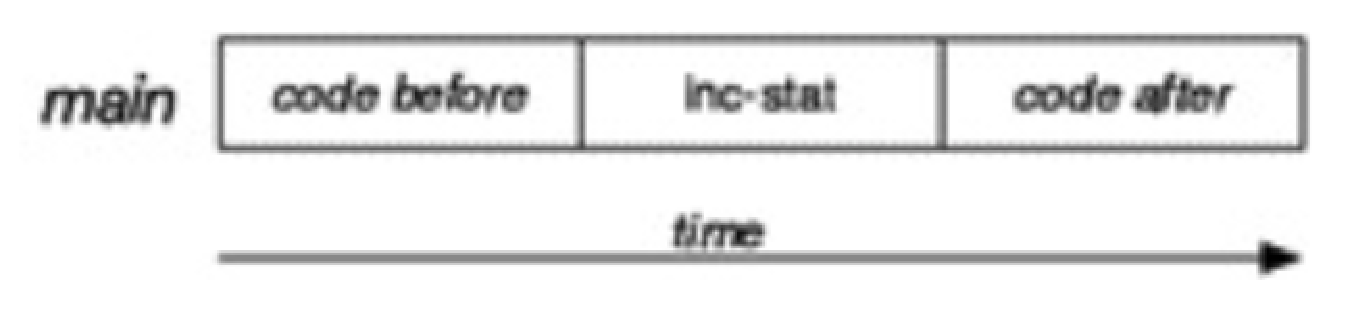
\includegraphics[width=10cm]{fig_05_001.eps}

この作業をバックグラウンドのスレッドに移すために、Clojureに含まれる\texttt{future}関数を使用します。

\begin{lstlisting}[numbers=none]
(future (inc-stat :pageview))
\end{lstlisting}

\texttt{future}関数はボディを受け取り、Clojure自身が維持するバックグラウンドのスレッドプールでそのボディを呼び出す。図にその違いを見ることができます。

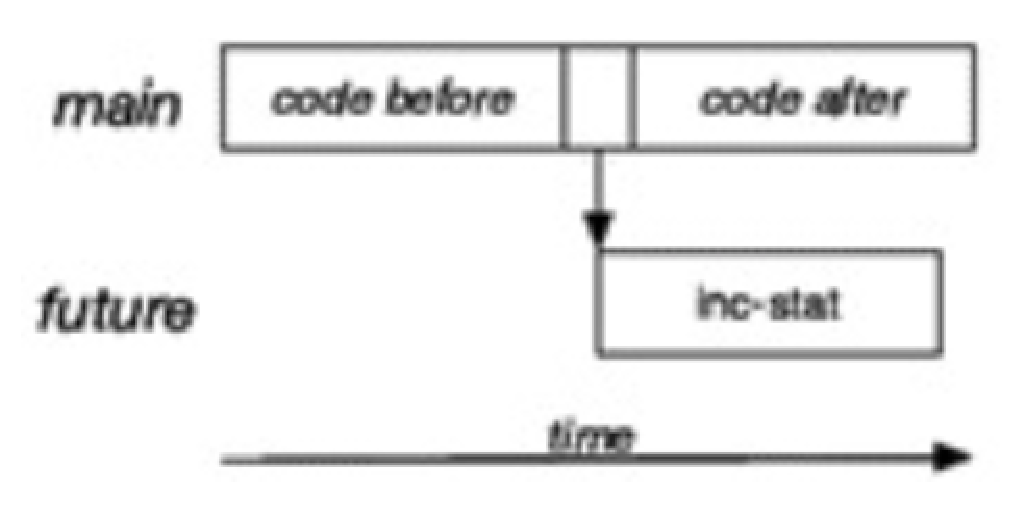
\includegraphics[width=8cm]{fig_05_002.eps}

また、\texttt{future-call}を使用すると、ボディを渡す代わりに引数のない関数を非同期で呼び出すことができます。どちらの関数も\texttt{java.lang.Future}オブジェクトを返し、それを使って非同期の活動を制御したり検査したりすることができます。\texttt{future-cancel}関数はその実行をキャンセルし、\texttt{future-done?}と\texttt{future-cancelled?}はその状態についての情報を与えてくれます。

しかし、独立した統計値増加メッセージをリモートサービスに大量に送信するのは非効率的だと思われます。送信前にいくつかのインクリメントメッセージをバッチ処理する方がより理にかなっています。そのためには、非同期かつステートフルである必要がある。


\subsection{非同期とステートフル}

第4章「状態、アイデンティティ、変化」では、Clojureの状態コンテナであるvar、atom、refを検討しました。もう一つの状態コンテナであるagentの紹介は、今まで遅らせました。

他のステート・コンテナと同様に、agentは不変の値を保持し、同じ更新モデルを使用して変更されます。他のコンテナとは異なり、agentは非同期に更新されます。

メトリクス・コレクターを考えてみましょう。ある統計量のカウンターをagentに保持することにしましょう。

\begin{lstlisting}[numbers=none]
(def pageview-stat (agent 0))
\end{lstlisting}

agentの更新ごとにリモートサービスを呼び出すのではなく、10回目の更新(agentの状態が10で割り切れる回数に達したとき)ごとに呼び出すことにします。これは、ウォッチ(すべてのステートコンテナで動作する)を使えば簡単にできます。


\begin{lstlisting}[numbers=none]
(add-watch
  pageview-stat
  :pageview
  (fn [key agent old new]
    (when (zero? (mod new 10))
      (remote-send key new))))
\end{lstlisting}







 % Push Waiting to the Background
\section{キューとワーカー}

多くのプログラムは、その全体または一部をタスク処理系として見ることができます。タスクとは、通常、外部からの要求に対応する作業の単位です。ウェブアプリケーションは、ウェブページを作成するためのリクエストを受け取ります。ウェブサービスは、APIコールを処理するリクエストを受け取ります。バッチプログラムはディスクやデータベースからファイルを読み込んで、それぞれを適切に処理する。これらの一般的なパターンはすべて、ワーカーのプールに委託された作業のキューとしてモデル化することができます。

キューは、タスクの順序付けと保持を行い、ワークが到着する場所と処理される場所を切り離します。ワーカープールでは、異なる特性を持つワーカーのプールを作成し、並行処理や、作業の管理・監視に使用するポリシーを制御することができます。その制御により、自由に使えるハードウェアをフルに活用することができるのです。

Clojureはキューとワーカーのためのいくつかのツールを提供しますが、Javaですでに利用可能な高品質のツールを再発明することも避けます。Clojureで既に見てきた部分から、キューとワーカープールをどのように作成できるか考えてみましょう。

\subsection{組み立てが必要}

第1章Model Your Domainでは、Clojureの永続キューを使用して、FIFOデータに対してリストやベクターよりも効率的なアクセスを提供しました。しかし、これはシングルスレッドのコンテキストで行われました。永続的なキューでは、キューを変更するたびに、更新されたバージョンが返されます。もし複数のスレッドがキューを共有するならば、それら全てが同じインスタンスを共有する必要があります。そのため、(atom や ref などの) 状態管理構造体か、状態管理型のキュー実装のいずれかが必要になります。

1つのオプションは、キューの両端が安定したアイデンティティを維持するように、Clojureのアトムまたは参照に永続的なキューをラップすることです。アトムでこれを行おうとすると、アトムの\texttt{swap!}関数がアトムの新しい値(私たちの場合はキュー)を返すだけで、ポップした値を返さないことに気づきます。このため、この種のキューからステートフルな方法でアイテムを取り出すことは困難です。

refオプションはより有望に見えます。このように実装できるだろう。


\begin{lstlisting}[numbers=none]
(defn queue
  "新しいステートフルキューの作成"
  []
  (ref clojure.lang.PersistentQueue/EMPTY))

(defn enq
  "qのitemを待ち受ける"
  [q item]
  (dosync
    (alter q conj item)))

(defn deq
  "qからitemを取り出す(なければnil)。"
  [q]
  (dosync
    (let [item (peek @q)]
      (alter q pop)
      item)))
\end{lstlisting}

しかし、このキューはブロックしない! 通常、キューが空でデータの到着を待っているときにコンシューマが \texttt{deq} でブロックすることを望みますが、この実装では \texttt{nil} を返すだけで、コンシューマが繰り返しポーリングすることを要求されます。この理由から、Clojureの永続的なキューは、通常、スレッド間で仕事のキューを管理するための良いツールではありません。

代わりに、キューとワーカーに対するJavaのサポートに注目する必要があります。これは、Javaライブラリが多種多様な動作に対して強力なサポートを持っている分野です。

\subsection{Javaキュー}

キューとワーカーをサポートするJavaクラスのほとんどは、\texttt{java.util.concurrent}パッケージで見つけることができます。Javaは多くのブロッキングキュー実装(すべて\texttt{java.util.concurrent.BlockingQueue}の実装)を提供し、それらはClojureから簡単に使用することができます。

Java のキュー実装の主な違いの1つは、データのバッファリング方法です。例えば、\texttt{LinkedBlockingQueue}はオプションで境界付きバッファを提供し、\texttt{ArrayBlockingQueue}は境界付きバッファを提供し、\texttt{SynchronousQueue}はバッファを全く提供しません。\texttt{LinkedTransferQueue} は、\texttt{SynchronousQueue} のハンドオフ機能と、オプションで制限されたバッファを組み合わせています。

これまで述べてきたすべてのキューは FIFO 順で値を提供しますが、Java は項目を並べ替えるキューも 2 つ提供します。\texttt{PriorityBlockingQueue} は、優先度の高い項目をキューの先頭にバブリングします。\texttt{DelayQueue}は、遅延のあるメッセージを受け取り、遅延の期限が切れたものだけを利用できるようにします。

Bounded buffer queue は、producer が満杯のバッファに遭遇したときに、カスタマイズする機会も提供します。Java のブロッキングキュー API では,ブロッキング,タイムドブロッキング,特別な値の返送,例外の発生が可能です.

\texttt{put} や \texttt{take} などの \texttt{BlockingQueue} メソッドは、通常の Java interop メソッド呼び出しで呼び出すことができます。それでは、いくつかのメッセージをキューにプッシュしてみましょう。

\begin{lstlisting}[numbers=none]
(ns ch5.jqueue
  (:import [java.util.concurrent LinkedBlockingQueue]))

(defn pusher [q n]
  (loop [i 0]
    (when (< i n)
      (.put q i)
      (recur (inc i))))
    (.put q :END))

(defn popper [q]
  (loop [items []]
    (let [item (.take q)]
      (if (= item :END)
          items
          (recur (conj items item))))))

(defn flow [n]
  (let [q (LinkedBlockingQueue.)
        consumer (future (popper q))
        begin (System/currentTimeMillis)
        producer (future (pusher q n))
        received @consumer
        end (System/currentTimeMillis)]
    (println "Received:" (count received) "in"
             (- end begin) "ms")))
\end{lstlisting}

\texttt{pusher}関数は、キューに\texttt{n}個の数値をプッシュし、最後に完了を知らせる\texttt{:END}メッセージを送ります。\texttt{popper}関数は同じキューから\texttt{:END}メッセージを受け取るまでメッセージを引き離します。これらの関数は両方ともバックグラウンドのスレッドプールで実行される \texttt{futures} で実行されます。

しかし、どのスレッドがこれらの\texttt{future}を実行するかは制御できません。Clojureのfutureとagentは非同期実行のための比較的簡単なAPIを提供しますが、監視と制御が多少損なわれます。その代わりに、多くのスレッド上で作業を実行するためのJavaのビルトインサポートを使用することができます。

\subsection{スレッドの作成}

Javaには、スレッドのファクトリー(\texttt{ThreadFactory})と、キューとワーカープールの組み合わせ(\texttt{ExecutorService})を表現するインタフェースが用意されています。

このように、プロセッサ数に応じた大きさの計算スレッドの固定プールを作成することができます。


\begin{lstlisting}[numbers=none]
(import '[java.util.concurrent Executors])

(def processors (.availableProcessors (Runtime/getRuntime)))

(defonce executor (Executors/newFixedThreadPool processors))

(defn submit-task [^Runnable task]
  (.submit executor task))
\end{lstlisting}

Javaでは、\texttt{Runnable}または\texttt{Callable}インタフェースを用いて実行可能なタスクを表現します。役に立つことに、すべてのClojure無引数関数はこれらのインターフェイスを実装しています。タスク(任意のClojure関数)は、呼び出すために\texttt{ExecutorService}に渡すことができます。したがって、リクエストのストリームをタップして、それらを実行のためのタスクとして送信するのは簡単です。

Java 5で追加されたJavaエグゼキュータは、当時一般的だった4~8コアのマシンで粗視化されたタスク並列をサポートするように設計されています。しかし、マシンのコアが増えるにつれ、1つのキューで待つことによる競合が、キューからアイテムを取得するワーカーのボトルネックとなりました。

この問題に対処し、他の計算パターンを利用するために、Java 7 では \texttt{fork/join} という新しいフレームワークが導入されました。\texttt{fork/join} は、より小さな粒度の細かい計算タスク、再帰的な計算、より多くのコアをサポートするように設計され、調整されています。\texttt{fork/join} は多数のワーカーキューを使用し、それらのキューが互いに仕事を「盗む」ことを可能にします。つまり、あるキューがやるべき仕事を使い果たした場合、別のキューの後ろからタスクを取り出し、キュー間の仕事のバランスを自動的に調整します。

\texttt{java.util.concurrent.ForkJoinPool} クラスは、Java のフォーク/ジョイン実装の主要なエントリポイントです。\texttt{ForkJoinPool}を構築すると、それは\texttt{ExecutorService}でもあり、同じようにタスクを投入することができます。しかし、Clojureは、Clojure開発者にとってより自然な方法で\texttt{fork/join}を活用するフレームワークを提供します。次に、そのフレームワークをいつ、どのように使用するかを見ていきます。 % Queues and Workers
\section{Reducerによる並列化}

Clojureでのデータ操作のほとんどは、シーケンスに適用される関数で指定されます。シーケンスとは(その定義から)、ある順序で値を並べた論理的なリストです。コアライブラリのシーケンス関数のほとんどは、1つのスレッドで、順番に、遅延して適用されます。コアの使用に関する章で推測されるように、この最後の詳細が問題なのです。

Reducer はシーケンシャルなデータに対する変換を表現する代替手段であり、シーケンス関数の合成と似たような感覚を持ちます。しかし、Reducerはfork/joinを使って変換を並列に実行することができます。

\subsection{シーケンスからReducerへ}

具体的な例で考えてみよう。ある運送会社が、今すぐ発送する必要のあるすべての商品に関するデータを持っている。各商品はドメインエンティティであり、出荷(shipping)クラスと重量(他の属性も含む)のキーを持つ。


\begin{lstlisting}[numbers=none]
{:id "230984234"
 :class  :ground
 :weight 10
 :volume 300}
\end{lstlisting}

現在のすべての地上出荷の総重量を計算するには、シーケンス関数を使って地上出荷だけを選択し、その重量を抽出し、それらを合計すればよい。


\begin{lstlisting}[numbers=none]
(defn ground? [product]
  (= :ground (:class product)))

(defn ground-weight [products]
  (->> products
       (filter ground?)
       (map :weight)
       (reduce +)))
\end{lstlisting}

Clojureでは、プログラムをシーケンスに対する一連のComposableな操作として簡単に表現することができます。チャンキングやトランジェントといった最適化によってサポートされる怠惰さは、大規模な商品リストに対してこれらの操作を効率的に実行することを可能にします。しかし、このコードでは1つのスレッドでしか処理を行いません。

Clojureは\texttt{pmap}と呼ばれる特別な並列版\texttt{map}を提供し、シーケンスの要素を取り、異なる要素を\texttt{future}でバックグラウンドスレッドに送ることで並列に作業を実行します。

しかし、ほとんどの場合、要素ごとに行うべきタスクは小さい(ここでは、マップから1つの属性を抽出するだけである)。\texttt{future}を呼び出すと、スレッド境界を越えて作業を渡し、結果を引き戻すための同期オーバーヘッドが追加されます。このオーバーヘッドに比べてタスクが小さい場合、\texttt{pmap} はシングルスレッド対応よりも遅くなることがあります。さらに、この使用例では、コードの\texttt{filter}や\texttt{reduce}の部分をまだ並列にしていません。

Clojureにはこの問題を解決する手段があります:reducerです。reducerは、データ変換を(シーケンスで行うのと同じように)一連の細かい操作として構成する方法を提供しますが、変換全体を実行しながら並列性を実現することができます。さらに、reducerはシーケンスで見られるような中間結果(後でガベージコレクションによって回収されなければならない)のほとんどを作成する必要がありません。

reducerは、削減可能なコレクションと削減関数の組み合わせで構成される。削減可能なコレクションとは、それ自身に対して可能な限り効率的に削減処理を行う方法を知っているコレクションにほかならない。削減関数は、削減中に結果を蓄積する方法を記述した関数である(ちょうど我々が通常\texttt{reduce}に渡す関数と同じである)。

シーケンスライブラリで既に使われているもの(\texttt{map}、\texttt{filter}、\texttt{mapcat}など)を反映したreducer操作が多数提供されています。これらの操作はreducerを受け取って返しますが、変換を実行するわけではありません。その代わり、これらの操作は単に新しい操作を考慮に入れて削減関数を修正するだけです。

変換を実行するために、\texttt{fold}という新しいreduceのような関数を呼び出す。図に示すように、\texttt{fold}はソースコレクションをグループに分割し、削減関数を使って各グループに対して削減を行い、結合関数を使って分割を結合する。現在のところ、並列でフォールドできるのは永続ベクトルとマップのみで、他のコレクションはすべて単一のシリアルリデュースにフォールバックします。このシリアル・リデュースは、中間結果を避けることができるため、同等のシーケンス・バージョンよりも効率的である可能性さえあります。 

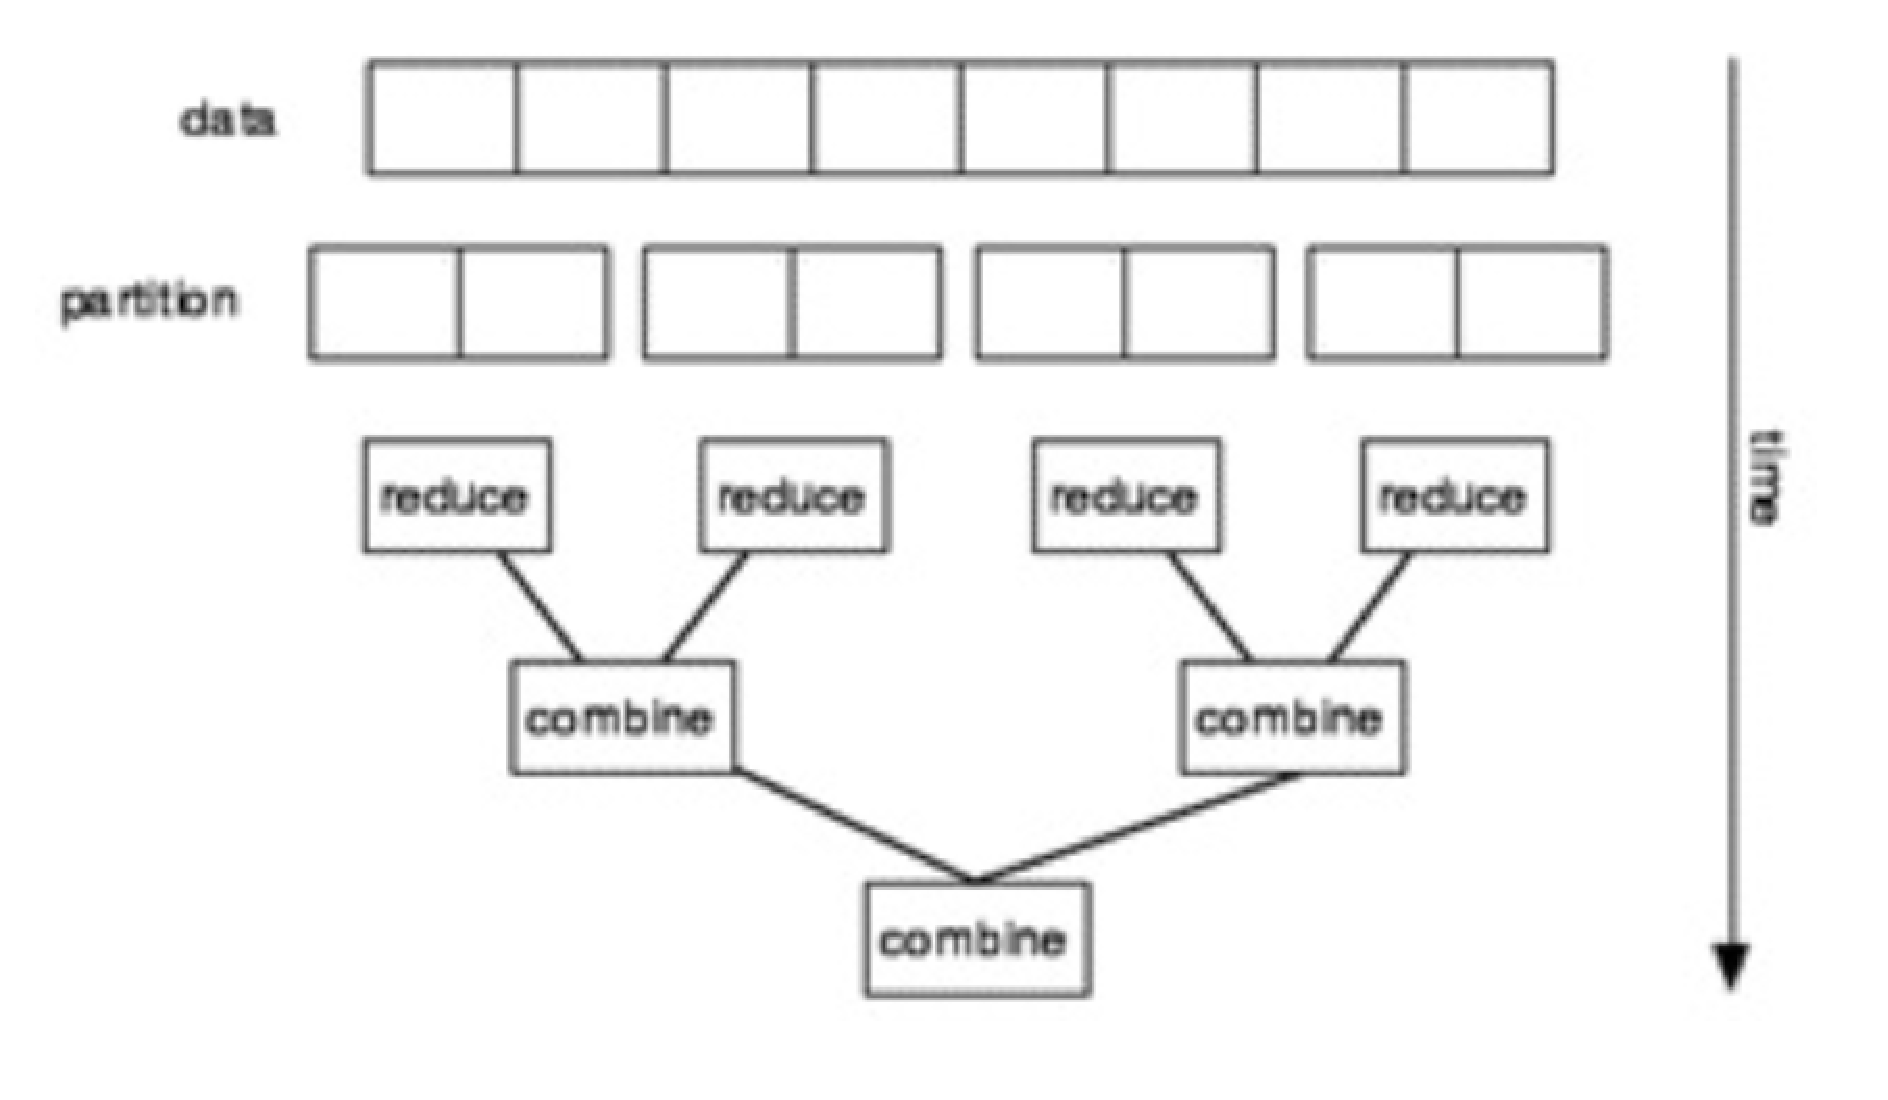
\includegraphics[width=12cm]{fig_05_005.eps}

先ほどの例に戻ると、\texttt{clojure.core.reducers}ライブラリを引き込み、reducerバージョンの関数を使って、ground-weightの計算を書き直すことができます。

\begin{lstlisting}[numbers=none]
(ns shipping.reducer
  (:require [shipping.domain :refer (ground?)]
            [clojure.core.reducers :as r]))

(defn ground-weight [products]
  (->> products
       (r/filter ground?)
       (r/map :weight)
       (r/fold +)))
\end{lstlisting}

この実装は、\texttt{clojure.core} 名前空間の代わりに \texttt{clojure.core.reducers} 名前空間の関数を使用する以外は、オリジナルバージョンと同様です。reducersの主な利点の1つは、他のアプローチと比較して、操作の構成可能な形状を維持することができることです。

フィルタとマップのリデューサーのバージョンは、元の積のベクトルに対して変換を実行しないことを思い出してください! 最終的に\texttt{fold}を呼び出すまで何も起こりません。この例では、reduceとcombineの両方のステージで同じ関数を使用する、最も単純なバージョンの\texttt{fold}を使用しています。

問題を再帰的に分割する並列計算では、以下のタイミングを決定する必要があります。分割と再合成は、単に作業を行うよりもコストがかかります。これは個々の計算の大きさに依存するため、最適な答えはない。\texttt{fold}関数では、分割サイズを指定することができ、デフォルトはグループあたり512要素(\texttt{+}などの単純な算術演算でうまくいくサイズ)です。より複雑な変換を行う場合は、より小さなパーティションサイズが有効でしょう。

今回はマルチコアマシンでのパフォーマンスを向上させるためにリデューサを使用するので、シーケンスとリデューサのパフォーマンスを比較してみましょう。

\subsection{Reducerの性能}

シーケンス版とリデューサ版を、どんどん大きな商品のベクターで走らせてみます。詳細を理解するために、2つのスケールでデータを見ることにします。次の図は、商品数(N)が32、128、512、2,048の場合の結果です。デフォルトのパーティションサイズは512なので、N <= 512の場合、実際には折りたたみは並列ではなく、1つのパーティションになります。これらのテストは、4つのハイパースレッドコア(8コアとして報告)を持つMacBook Proで実行されました。

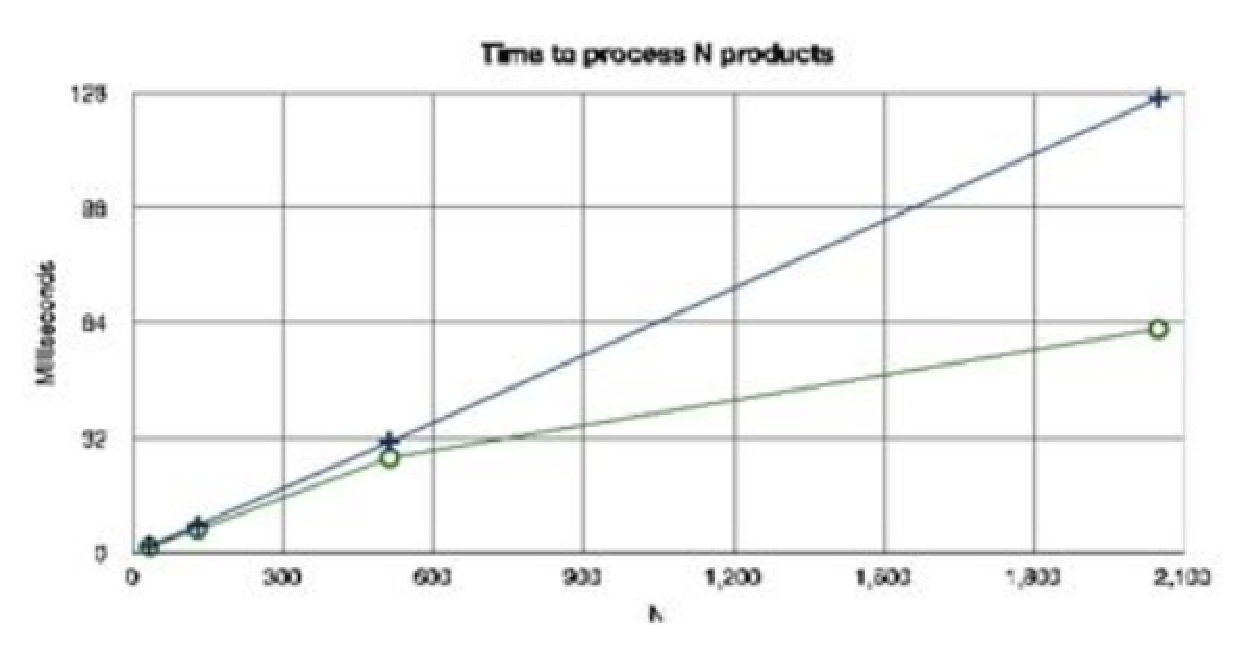
\includegraphics[width=10cm]{fig_05_006.eps}

予想通り、N=512まではシーケンス版とリデューサーの性能は同等である。しかし、パーティションサイズを超えると、シーケンス版はシングルスレッドですが、リデューサ版はデータをパーティションに分割し、異なるスレッドで並列実行されます。ここで一旦引いて、次の図にある3つのデータポイント(N=8,192, 32,768, 131,072)を追加して、Nの値が大きい場合の影響を見てみましょう。

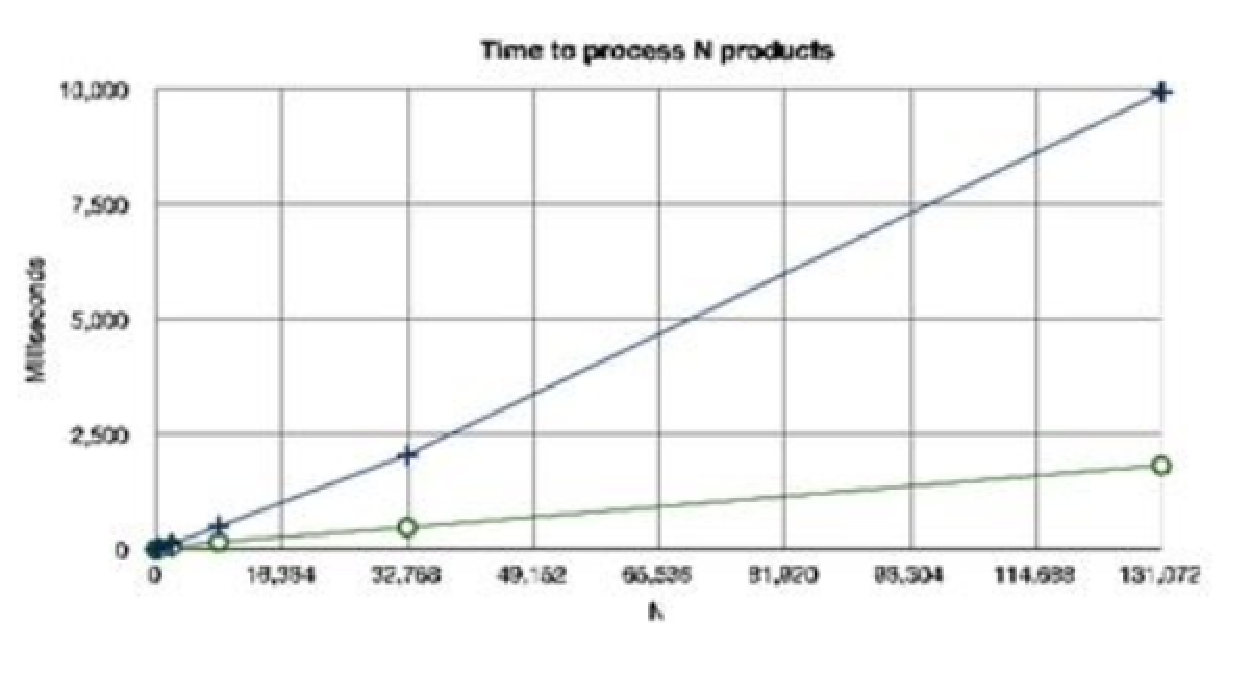
\includegraphics[width=10cm]{fig_05_007.eps}

Nが大きくなると、reducerの利点が明らかになる。reducerは4つの利用可能なコアに作業を分割するのに対し、シーケンスバージョンは1つのコアを使用するのである。さらに、reducer版ではゴミの発生が少ないので、ガベージコレクタの負荷が軽減されます。

reducerの主な利点の1つは、より多くのコアを持つマシンに移行したときに、同じコードがより速く実行されることです。マシンのコアの一部をオフにすることで、その違いをシミュレートすることができます。N=131,072 を固定し、コア数を変化させながら、シーケンスとreducerのテストを再実行してみましょう。このテストでは、ハイパースレッディングもオフにして、その影響を排除しています。

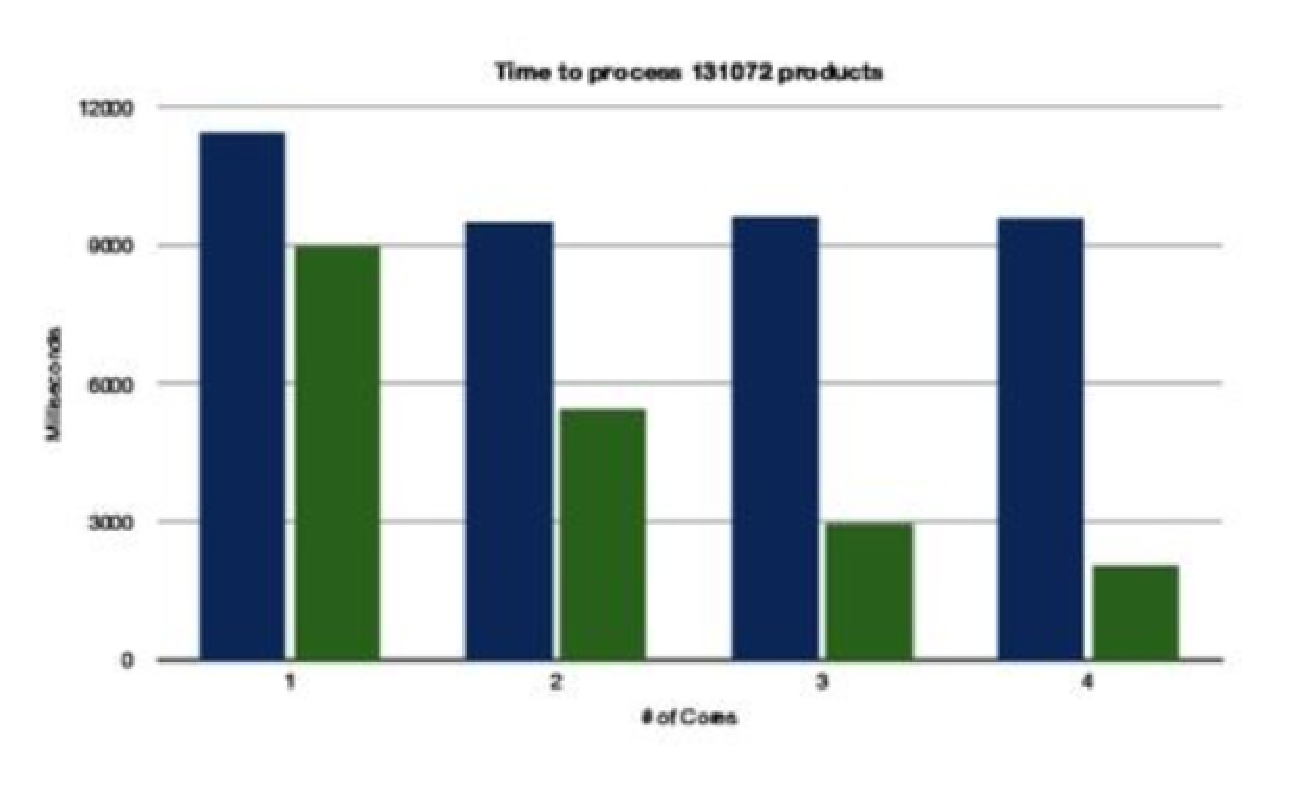
\includegraphics[width=10cm]{fig_05_008.eps}



前の図で、シーケンス版の性能はコア数に関係なく事実上同じであることがお分かりいただけると思います。シングルコアの場合は、ガベージコレクションやその他のマシン上の作業も唯一のコアを使用するため、特に悪化します。しかし、reducer版では、明らかに余分なコアの恩恵を受けており、同じコードが自動的に高速化されます。8コアや16コアのサーバーに移行すれば、このコードはさらに高速になると推測できます。

reducerを使うときは、データの大きさ、パーティションごとの作業の大きさ、想定するコア数を考えることが重要です。要素数がパーティションサイズより小さいときは、シングルスレッドになります(それでも穏やかな効果が見られるかもしれません)。パーティションサイズを超えると、reducerはマルチスレッドになりますが、オーバーヘッドが発生するため、コア数の倍数にはならない可能性があります。

もう1つのキーは、並列折りたたみ可能なコレクションは(現在ではもっと追加されるかもしれませんが)永続ベクトルと永続マップだけであることです。他のすべてのコレクション(およびシーケンス)は、1つのパーティション上のリダクションにフォールバックされます。このリダクションはより高速になる可能性がありますが、マルチスレッドにはなりません。

Reducerは、シーケンスライブラリの使いやすさと、fork/joinのマルチスレッド性能を併せ持つもので、両者の良いとこ取りのようなものです。reducers を最大限に活用するには、処理量が多く、データが折りたたみ可能なベクトルやマップとして存在する場合に限定して使用するようにしましょう。 % Parallelism with Reducers
\section{プロセスで考える}

これまで、一回限りの非同期(\texttt{future}や\texttt{promise})、粗粒度のタスク並列、細粒度のデータ並列のためのコアの使い方をみてきました。しかし、時には並列性よりも並行性に興味を持つことがあります。つまり、プログラムを一連の同時実行スレッドとして設計する能力です。また、これらのスレッド間で、一度だけでなく、時間の経過に伴う一連の値として、値を伝達したいと思うこともあるはずだ。

\texttt{core.async}ライブラリは、このようなニーズに対する回答として作成された。当初はClojure自体の一部として構想されましたが、最終的にはコア言語よりも迅速な進化を可能にするために、独立したライブラリとしてリリースされました。\texttt{core.async}ライブラリは、goブロック(独立した実行スレッド)とチャネル(ある場所から別の場所に値を渡す手段)という2つの中心的な概念を提供します。次に、これらの使い方を探ります。


\subsection{チャネル}

チャネルは、プログラムの2つ以上の部分の間で一連の値を時間的に伝達するための待ち行列のような手段です。チャネルは、スレッド間で作成したり受け渡ししたりすることができます - ステートフルです。

チャネルは、チャネル内の値を保持するためにバッファを使用します。デフォルトでは、チャネルはバッファなし(長さゼロ)で、Javaの\texttt{SynchronousQueue}に似ています。バッファされていないチャネルは、producer と consumer の両方がチャネルに値を渡すことができるようになるまでブロックされます。\texttt{core.async} ライブラリは,固定長のバッファ,ドロップバッファ(新しいデータが一杯になったらドロップする),スライディングバッファ(古いデータが一杯になったらドロップする)も提供します.

\texttt{core.async} でチャネルを作成するには、\texttt{chan} 関数を使用します。以下は、異なるバッファタイプとサイズのチャネルを作成する例です。

\begin{lstlisting}[numbers=none]
(require '[clojure.core.async :refer
 (chan dropping-buffer sliding- buffer)])

(chan) ;; unbuffered (length=0)
(chan 10) ;; buffered (length=10)
(chan (dropping-buffer 10)) ;; drop new values when full
(chan (sliding-buffer 10)) ;; drop old values when full
\end{lstlisting}

どんな典型的なClojure値でもチャネルに入れることができ、相手側に伝達されます。1つの例外は \texttt{nil} で、これはチャネルが閉じられ、それ以上データが残っていないことを示すために使用される特別な値です。チャネルは,\texttt{close!}関数で閉じられます.

チャネルに対する最も重要な操作は \texttt{put} と \texttt{take} の 2 つであり、それぞれコンテキストや用途に応じていくつかの形式があります。通常のスレッドからチャネルを使用する場合、\texttt{put} 演算子は \texttt{>!!}、\texttt{take} 演算子は \texttt{<!!} となります。以下は,チャネルを作成し,そこに値を入れ,取り出す例です.

\begin{lstlisting}[numbers=none]
(require '[clojure.core.async :refer (chan <!! >!!)])

(def c (chan 1))
(>!! c "hello")
(println (<!! c))
\end{lstlisting}

前述のコード例では、\texttt{put}と\texttt{take}の両方の操作を現在のスレッドから行っていますが、実際のプログラムでは、チャネルの両端は通常、異なるスレッドまたはコンポーネントから使用され、それらの間で値が送信されるようになっています。また、サイズ 1 のバッファを持つチャネルを作成したことにお気づきでしょうか。もしバッファのないチャンネルを使っていたら、この例では put の待ち時間がブロックされ、この例が完了するのを妨げていたでしょう。

\texttt{core.async} のチャネルは決して unbounded ではありません。これは、後で問題になるようなアーキテクチャ上の問題を避けるための、意図的な設計上の制約です。システム内の未束縛のキューは、予期せぬ負荷が積み重なり、最終的にはリソースを使い果たし、システムをクラッシュさせる場所となります。

その代わりに、\texttt{core.async}では、固定サイズを選択するか、バッファがいっぱいになったときに何をドロップするかのポリシーをインスタンス化することで、バッファの長さを制限することを要求します。固定サイズのバッファは、満杯のキューに追加しようとするとプロデューサーをブロックさせるので、バックプレッシャーを発生させます。これは、実稼働時ではなく、前もっての設計思考を促すものです。システムは、負荷がなくなるのを待つか、仕事を減らすことを受け入れるか、どの仕事をしないかを選択することによって、明示的にブロックに対処するように設計されていなければなりません。

チャネルを別のサブシステムの専用スレッドから完全に使用することも可能ですが、Goブロックから使用するのが一般的です。Goブロックを使うと、スレッドのプールで対応できる軽量な処理ループを作ることができます。

\subsection{Goブロック}

伝統的に、Java(またはClojure)プログラムは、プログラムの各部分の実際の処理を含むスレッド(実際のオペレーティング・システムのスレッドに対応する)を作成します。\texttt{core.async}ライブラリは、C. A. R. HoareのCommunicating Sequential Processes (CSP) [Hoa78]の遺産に基づく、異なる伝統に従います。

この研究の詳細については、ここでは触れません。重要なことは、プログラムをどのように構成するかについて、異なる方法で考えることを学ぶことです。スレッドは希少で高価な資源です。スタックスペースやその他の資源を消費し、起動も比較的遅いです。スレッドがI/Oのためにブロックされると、これらのシステムリソースを浪費することになります。

その代わりに、\texttt{core.async}は、スレッドプールにマッピングされ、作業の準備ができたときにだけ実行される軽量なプロセスという観点から考えることを推奨しています。チャネルへのメッセージの出入りを待つ間にブロックする代わりに、プロセスが再び実行できるようになるまで、これらのプロセスを停止させることができます。これによって、やるべきことがあるときだけプロセスを実行することができる。また、複数の I/O 操作にまたがって選択し、最初の操作が完了したときに処理を進めるという、興味深い新しい動作を実装することも可能です。

\texttt{core.async}では、これらのプロセスをGoブロックと呼んでいます(Go言語の同様の概念にちなんでいます)。goブロックの中ではチャネルを使いますが、\texttt{put}と\texttt{take}の操作は \texttt{<!} と \texttt{>!} です。

以下は、メッセージを受信し、それを表示する処理を行うgoブロックを作成する関数の例です。

\begin{lstlisting}[numbers=none]
(require '[clojure.core.async :refer (go <!)])

(defn go-print
  "チャネル c からメッセージを取り出し、表示する。"
  [c]
  (go
    (loop []
      (when-some [val (<! c)]
        (println "Received a message:" val)
        (recur)))))
\end{lstlisting}

この例では、goブロックは軽量なプロセスとして実行されます。チャンネル操作(\texttt{<!} や \texttt{>!} など)に到達したとき、そのチャンネル操作が可能であれば実行を継続する。チャンネル操作が継続できない場合、go ブロックはパークされます。パークされたgoブロックはスレッドを消費せず、事実上、データを待つために中断された計算となります。チャネル操作が続行できるようになると、goブロックは実行を継続するために起動します。

Goブロックは、プログラムを潜在的な同時処理に分割するための素晴らしいツールです。\texttt{core.async}がgoブロックとチャネルで特によくサポートする使用例は、データ変換ステージのパイプラインを構築することです。

\subsection{パイプライン}

\texttt{core.async}ライブラリは,2つのチャンネルを並列変換ステージで接続するための関数群,すなわち\texttt{pipeline},\texttt{pipeline-blocking},\texttt{pipeline-async}を提供します.このパイプライン関数は、入力チャネルから出力チャネルに値を移動しますが(より単純な\texttt{pipe}と同様)、重要な追加機能を提供します:トランスデューサの並列実行です。

この機能により、パイプラインはチャネルで区切られたデータ変換ステージを作成するのに適しています。並列実行により、データパイプラインを線形に記述しながら、コアをフル活用することができます。各トランスデューサステージは多くの変換を組み合わせることができるため、どのように並列化するか、どこでチャネルを分離するのが有効か、多くの選択肢があります。

例えば、ソーシャルメディアのメッセージのストリームを処理するシステムを考えてみましょう。トランスデューサーとして定義された一連の変換を提供することができます。

\begin{lstlisting}[numbers=none]
;; メッセージを単語の集合に解析する
(def parse-words
  (map #(set (clojure.string/split % #"\s"))))
;; 単語を含むメッセージをフィルタリングする
(def interesting (filter #(contains? % "Clojure")))
;; 異なる単語リストに基づいて感情を検出
(defn match [search-words message-words]
  (count (clojure.set/intersection search-words
                                   message-words)))
(def happy
  (partial match
           #{"happy" "awesome" "rocks" "amazing"}))
(def sad (partial match #{"sad" "bug" "crash"}))
(def score (map #(hash-map :words %1
                           :happy (happy %1)
                           :sad (sad %1))))
\end{lstlisting}

これらのトランスデューサは、入力ストリームから出力ストリームまで1段のパイプラインで一緒に構成することができます。


\begin{lstlisting}[numbers=none]
(defn sentiment-stage
  [in out]
  (let [xf (comp parse-words interesting score)]
    (async/pipeline 4 out xf in)))
\end{lstlisting}

これは、最大4つの並列スレッドで \texttt{in} と \texttt{out} を接続し、それぞれが結合されたトランスデューサの変換を処理します。しかし、センチメント分析が行われている間に、アーカイブへのロギングなど、別のパイプラインステージで発生する可能性のある他の分析があるかもしれません。その場合、このステージを2つに分割し、センチメント解析の前に新しい中間チャネルを作成することができます。

\begin{lstlisting}[numbers=none]
(defn interesting-stage
  [in intermediate]
  (let [xf (comp parse-words interesting)]
    (async/pipeline 4 intermediate xf in)))

(defn score-stage
  [intermediate out]
  (async/pipeline 1 out score intermediate))

(defn assemble-stages
  [in out]
  (let [intermediate (async/chan 100)]
    (interesting-stage in intermediate)
    (score-stage intermediate out)))
\end{lstlisting}

現在では、受信したメッセージをすべて受け取り、興味深いものだけを出力する第一ステージ(最大4スレッドを使用)と、興味深いメッセージを受け取り、スコアをつける第二ステージがあります。量が少ないので、第2ステージの並列度を1スレッドに減らすことができます。これらのステージを組み立てると、中間メッセージチャネルを他の目的に使用する機会も得られます。

トランスデューサーはコンポーザブルなので、1つのステージに積み重ねることもできますし、ステージをまたいで分割することも可能です。各ステージの並列度は独立して変化させることができる。これは、効率的なデータ処理パイプラインを構築するための強力な技術です。パイプラインは、きめ細かなデータ並列処理の性能を犠牲にすることになりますが、より柔軟なアーキテクチャを実現することができます。


 % Thinking in Processes
\section{まとめ}

ムーアの法則に従ってトランジスタ数が増え続けるのは確かだが、それに伴うクロック速度の向上はもはや期待できない。その代わり、チップあたりのコア数は増え続けている。これからは、より多くのコアが利用可能になったときに、それを自動的に活用できる言語が求められているのです。

これまで、より多くのコアを利用して、より多くの作業を行うことができる分野をいくつか取り上げてきました。まず、futureを使ってバックグラウンドスレッドで非同期処理を行うことを考えてみました。Futuresは、非同期タスクを実行し、場合によってはその結果を通信で返す必要がある場合に、最初に選択すべきものです。もし、複数の値や非同期タスクの任意の場所からの配信が必要な場合は、promiseを使用してください。非同期タスクが状態を保持する必要がある場合(シミュレーションなど)、agentが最適です。

もし、あなたのシステムが仕事やリクエストの受信キューとして構成されているなら、その仕事をキューで受け入れ、ワーカスレッドのプールに送って処理する必要があります。そのためには、標準的なJavaライブラリのツールを使って、キュー、スレッド、エグゼキュータを使ってシステムを構成してください。

データが大きなベクトルやマップになっている場合は、reducerを使ってデータセット全体に対して並列に動作するように計算を構成する必要があります。reducerはシーケンス関数に期待されるような複合化能力を持ちながら、マシンの全コアをフルに活用することができ、中間オブジェクトを避けることでガベージコレクションを最小限に抑えることができます。

並行処理についてまだ調べていないことのひとつに、成長するシステムをいかにして断片化するかがあります。コンポーネント間の長寿命な接続を作成するために、再び core.async を活用することができます。次に、完全なアプリケーションを構築するために、これらのコンポーネントをどのように構築するかに焦点を当てます。


Footnotes
[19]
http://dl.acm.org/citation.cfm?doid=828.833 % Wrapping Up